% file: jupiter-tlaplus.tex

\documentclass[tikz]{standalone}
\usetikzlibrary{positioning, fit}

\newcommand{\red}[1]{\textcolor{red}{#1}}
\newcommand{\blue}[1]{\textcolor{blue}{#1}}
\newcommand{\hl}[1]{\fcolorbox{yellow}{yellow!60}{#1}}

\begin{document}
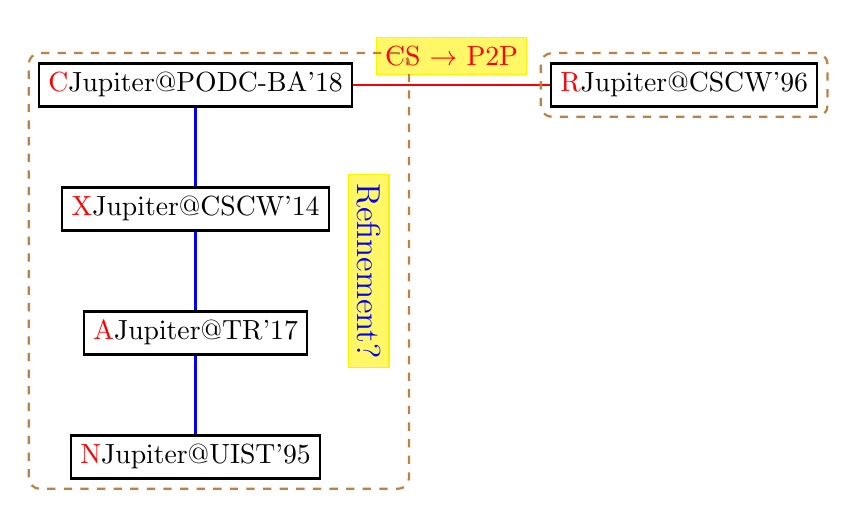
\begin{tikzpicture}[every node/.style = {draw, thick},
  node distance = 1.0cm and 2.5cm,
  every edge/.style = {draw, thick, blue},
  txt/.style = {draw = none}]
  \node (cjupiter) [] {\red{C}Jupiter@PODC-BA'18};

  \node (xjupiter) [below = of cjupiter] {\red{X}Jupiter@CSCW'14};
  \node (ajupiter) [below = of xjupiter] {\red{A}Jupiter@TR'17};
  \node (njupiter) [below = of ajupiter] {\red{N}Jupiter@UIST'95};

  \node (rjupiter) [right = of cjupiter] {\red{R}Jupiter@CSCW'96};

  \path (cjupiter) edge (xjupiter)
	(xjupiter) edge node (refine) [sloped, above = 1.8cm, txt, font = \large] {\hl{\blue{Refinement?}}} (ajupiter)
  	(ajupiter) edge (njupiter)
	(cjupiter) edge[red] node[above, txt] {\hl{\red{CS $\to$ P2P}}} (rjupiter);

  % cs
  \node () [draw, dashed, brown, rectangle, rounded corners, fit = (cjupiter) (njupiter) (refine)] {};
  % p2p
  \node () [draw, dashed, brown, rectangle, rounded corners, fit = (rjupiter)] {};
\end{tikzpicture}
\end{document}
